\chapter*{Introduction}
\label{cap:introduction}
\addcontentsline{toc}{chapter}{Introduction}

In recent years, cases have been presented of people who claimed to be able to
play a game using only a headset and their thoughts, without pressing buttons.
However, these articles provide scarce information in this regard, proving to
be unreliable. In the event that playing a game ``with thoughts'' is possible,
it would represent a major breakthrough in accessibility systems, as well as a
novel and attractive approach for the video game environment.

Despite the existence of such examples, brain-computer interfaces
(\textit{Brain-Computer Interfaces}, BCI) have experienced verifiable and
significant growth. Advances have been made both in research, achieving
artificial intelligence (AI) models with very promising results, and in
applications related to accessibility and human-computer interaction. The
visible progress is encouraging; however, a problem exists: all these advances
usually require a large budget or cumbersome EEG\footnote{EEG
(Electroencephalography): a non-invasive recording technique that allows the
measurement of the electrical activity of the brain through electrodes placed on
the scalp.} signal reading headsets.

This work focuses on the design and implementation of a system capable of
interpreting EEG signals in real time and translating them into usable actions
within different video games. To this end, it is proposed to develop a modular
architecture oriented towards the continuous acquisition of signals, their
processing, the classification of the input, and the translation of the
classification into a real-time action in a video game.

The proposal involves different challenges due to the nature of EEG signals:
the presence of noise in the waves, their variability, and the difficulty of
obtaining stable predictions in real time, among others.

In addition to the processing \textit{pipeline} itself, it is proposed to
design different games specifically adapted to the limitations and
characteristics of the proposed BCI system. These environments will allow the
evaluation of the system's behavior in dynamic and interactive situations,
facilitating both the analysis of technical performance and the user's
experience.

\section*{Motivation}
\addcontentsline{toc}{section}{Motivation}

If a video game could be controlled with thoughts, it would not only be of
great help to people with reduced mobility, allowing them to play comfortably,
but it would also be of great interest to the rest of the world as a more
immersive and novel game concept, in addition to the attractive idea of
controlling something without moving or giving voice commands. Controlling a
game with thoughts would open the doors to a new level of gameplay and interface
between humans and machines.

Brain-computer interfaces are one of the most interesting lines of research
within the field of human-computer interaction, due to the possibilities they
offer both in accessibility and in new forms of digital interaction. The
possibility of controlling a system through brain activity opens the door to
applications oriented towards people with reduced mobility, assistance systems,
and new interactive experiences.

However, many of the existing developments are achieved in highly controlled
laboratory environments or in solutions with a high economic cost, using devices
that are poorly accessible to the average user. Furthermore, many systems fail
to transfer the results obtained in controlled tests to real-time interactive
applications, especially in dynamic contexts such as video games.

Added to this is the inherent complexity of EEG signals. These turn out to be
excessively variable, are highly sensitive to noise, and generate predictions
that can fluctuate considerably within very small time intervals. As a
consequence, building a stable and functional system poses a challenge both
from a technical standpoint and from interaction design. Even when using an
almost infallible prediction model, assistance mechanisms are needed to adjust
decision-making in a controlled manner.

The main motivation of this work stems from the interest in exploring to what
extent it is possible to develop a BCI system that allows controlling a video
game and operates using hardware that is relatively accessible, all things
considered.

Due to the advances in AI to date and studies related to BCIs, it is believed
possible to achieve promising results with a well-planned and implemented
system, and a relatively accessible EEG headset.

\section*{Objectives}
\addcontentsline{toc}{section}{Objectives}

The main objective of this work is to develop an accessible brain-computer
interface (BCI) system, capable of interpreting motor
imagery\footnote{Motor imagery: a brain-computer interface paradigm based on the recognition of imagined movements.} (MI) signals in real time and applying them to the control of interactive systems and video games.

To achieve this main purpose, the following general objectives are proposed:

\begin{itemize}

    \item \textbf{Transform MI-based EEG signals into commands applicable to a video game:}
          Acquire, process, and interpret EEG signals using artificial intelligence techniques to generate actions applicable to an interactive environment.

    \item \textbf{Design a gaming experience adapted to the limitations of BCI systems:}
          Develop decision filtering and assistance mechanisms to compensate for the inherent instability of EEG signals and offer a smooth and pleasant gaming experience for the user.

    \item \textbf{Evaluate viability and playability in real users:}
          Carry out real-time experiments to validate the accuracy, latency, and user experience of the complete system.

\end{itemize}

More specifically, as a means to achieve these general purposes, the following
specific objectives are required:

\begin{enumerate}[label=\Alph*.]
    \item \textbf{Perform data capture with the EEG headset:} Obtain a custom EEG reading with timestamps.
    \item \textbf{Devise a method for preprocessing and dividing the signal:} Learn to handle the raw input from the EEG headset to obtain something manageable. Design and evaluate different techniques to improve the quality of EEG signals and divide them.
    \item \textbf{Choose and adapt a classification model:} Research and compare classification models to select the one with the best results. Analyze the \textit{performance} both with public \textit{datasets} and with the EEG recordings performed in this project.
    \item \textbf{Create a specific dataset for the model:} Devise a protocol and apply it to different users to achieve a structured and professional \textit{dataset}. This will serve to perform tests and evaluate the model.
    \item \textbf{Concurrently receive and classify EEG signals:} Propose an implementation capable of constantly receiving EEG signals from the headset and processing them.
    \item \textbf{Group classifications in real time:} Analyze methods to transform the constant flow of predictions into something continuous and useful.
    \item \textbf{Design video games that can be controlled with the achieved predictions:} Think of and implement video games whose controls are compatible with the predictions and whose speed is adaptable or corresponding to the system's latency.
    \item \textbf{Propose assistance mechanisms to compensate for prediction errors:} Devise algorithms capable of correcting (in a controlled manner) the decisions predicted by the model before executing them in the video game.
    \item \textbf{Organize a clear structure for the experiments:} Decide on a structure to follow for real-time video game experiments.
    \item \textbf{Develop the questionnaire to be completed by users:} The questionnaire will serve to measure satisfaction levels, the sensation of control over the system, and the overall experience.
    \item \textbf{Gather people for the experiment:} Call upon individuals willing to test the developed system to obtain results from real users.
    \item \textbf{Study the results obtained in the experiment:} Analyze the data collected from the real-time experiments.
\end{enumerate}

\section*{Tools used}
\addcontentsline{toc}{section}{Tools used}
During the development of the project, different tools have been used, each
oriented towards a specific purpose within the different phases of the project.

\begin{itemize}
    \item \textbf{BrainAccess\footnote{\url{https://www.brainaccess.ai/wp-content/uploads/2022/04/UserManualCAP.pdf}} MIDI 16-channel electroencephalograph:} EEG signal acquisition device used for collecting data from the participants.

    \item \textbf{Visual Studio Code\footnote{\url{https://code.visualstudio.com}}:} integrated development environment (IDE) used both for implementing the software in Python and for preparing this document in \LaTeX.
    
    \item \textbf{Anaconda\footnote{\url{https://www.anaconda.com}}:} Python environment management platform used for dependency control and package conflict resolution.

    \item \textbf{GitHub\footnote{\url{https://github.com}}:} version control platform that has enabled parallel work and the maintenance of a project change history.
    
    \item \textbf{Google Gemini\footnote{\url{https://gemini.google.com}}:} Google's artificial intelligence model used for implementing the video games to be tested.

    \item \textbf{Google Forms\footnote{\url{https://forms.google.com}}:} used for preparing and distributing a questionnaire intended for the participants of the game experiments.
    
    \item \textbf{OneDrive\footnote{\url{https://onedrive.live.com}}:} used for sharing and storing documentation, video recordings, and other relevant project files.
    
    \item \textbf{Camcorder:} high-resolution recording device used to register participants during gaming sessions.
\end{itemize}

\section*{Work plan}
\addcontentsline{toc}{section}{Work plan}

A work plan oriented towards the achievement of the defined objectives has been
followed, seeking to maximize efficiency throughout the development of the
project. Strategic decisions were made to parallelize independent tasks
whenever possible, so that no team member was left without an assigned task and
unproductive time was minimized. The temporal planning is reflected in the Gantt
chart (see Figure~\ref{fig:diagrama_gant}), where the distribution of the
different objectives over time can be visualized.

The tasks that required the most time were those related to device data
acquisition, carried out in parallel with the research and development of
signal preprocessing and the search for predictive models, a trend that is
subsequently repeated with the development of the video games and the real-time
system architecture. It is worth noting that the pace of development
progressively accelerated as deeper knowledge of the device's SDK was gained and
conflicts arising with certain Python libraries were resolved.

\begin{figure}[h]
    \centering
    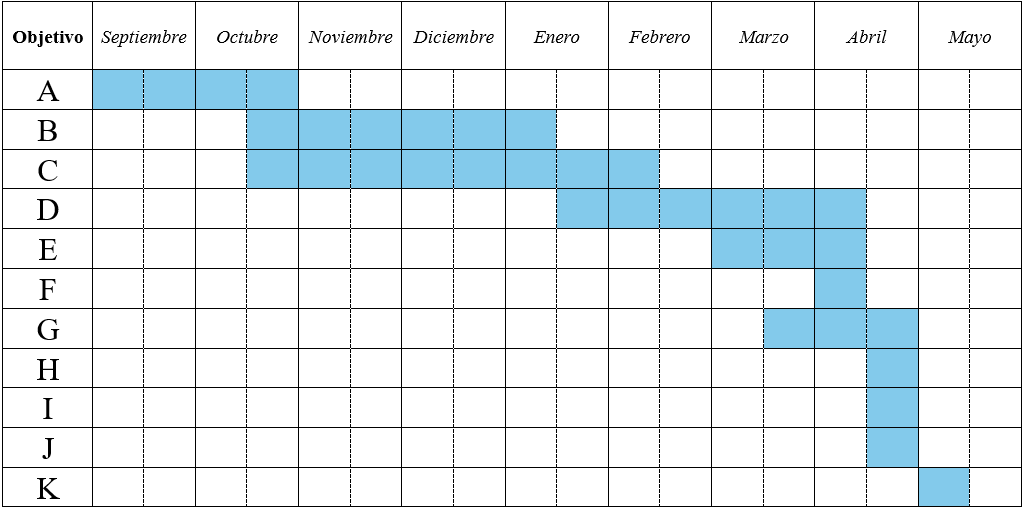
\includegraphics[width=1\textwidth]{Imagenes/Bitmap/Diagrama_Gantt.png}
    \caption{Gantt chart of the project's work plan. It stands out that the tasks linked to device data acquisition concentrated the greatest time load at the beginning of the project.}
    \label{fig:diagrama_gant}
\end{figure}


\section*{Document structure}
\addcontentsline{toc}{section}{Document structure}

The document is structured into ten chapters organized as follows:

\begin{itemize}
    \item \textbf{Chapter~\ref{cap:introduccion}:} Contains the current introduction, which 
    presents the project's motivation, defines the specific objectives, 
    describes the tools used during development, and presents the 
    followed work plan.

    \item \textbf{Chapter~\ref{cap:estadoDeLaCuestion}:} Delves into the state of the art, 
    presenting the scientific areas involved in acquiring information 
    from the human brain, the techniques used to extract this information, 
    and the use of brain-computer interfaces in the field of video games. 
    Likewise, reference is made to similar work carried out by other 
    researchers and developers.

    \item \textbf{Chapter~\ref{cap:arquitecturaPipeline}:} Describes the architecture of the BCI system 
    developed for real-time use with video games, detailing the 
    components, modules, and mechanisms that make up its structure.

    \item \textbf{Chapter~\ref{cap:aplicacionBCI}:} Is dedicated to the application developed to 
    facilitate the tasks of recording, conducting experiments with 
    participants, visualizing sessions, and evaluating the motor imagery 
    predictive model on the recordings made.

    \item \textbf{Chapter~\ref{cap:tratamientoDatos}:} Covers everything related to EEG signal 
    preprocessing, including filtering, normalization, detection of 
    artifacts and low-quality data, as well as the description of the 
    predictive model used and the results obtained with the different 
    subjects who participated in the recording experiments.

    \item \textbf{Chapter~\ref{cap:experimentosPreliminares}:} Describes the process of conducting the 
    recording sessions, including the instructions provided to the 
    participants and the environmental conditions, both in the initial 
    pilot experiments and in the final recording experiments.

    \item \textbf{Chapter~\ref{cap:aplicacionAVideojuegos}:} Explains the development of the video games 
    integrated into the BCI system and their integration into the 
    application, also describing the different fault tolerance techniques 
    and assistance systems implemented to facilitate the control of the games.

    \item \textbf{Chapter~\ref{cap:experimentoTiempoReal}:} Describes the process of conducting the 
    real-time experiments with video games, detailing the environment, the 
    instructions provided to the participants, the metrics obtained, and 
    the questionnaire completed by the participants at the end of each session.

    \item \textbf{Chapter~\ref{cap:rt_resultados_y_analisis}:} Focuses on the analysis of the data collected 
    during the experiments, both the system metrics and the responses 
    obtained through the questionnaires described in the previous chapter.

    \item \textbf{Chapter~\ref{cap:conclusiones_y_trabajo_futuro}:} Develops the conclusions derived from the work 
    carried out and the results obtained, and identifies the lines of 
    future work.
\end{itemize}

Finally, the English versions of the \textbf{Chapters \hyperref[cap:introduction]{Introduction} and \hyperref[cap:conclusionsAndFutureWork]{Conclusions and future work}} are included, followed by the chapter on the personal contributions of each team member (\textbf{Chapter \hyperref[cap:contribucionesPersonales]{\textit{Contribuciones personales}}}), and lastly the bibliography.